\documentclass[a4paper]{ctexart}


\newcommand{\workingDate}{\textsc{2026 $|$ January $|$ 13}}
\newcommand{\userName}{JINGANG ZHAO}
\newcommand{\institution}{HENAN MEDICAL UNIVERSITY}
\newcommand{\diaryTitle}{NoteBooks} 

\usepackage{../assets/styles/handout_base}        % Core packages and basic theorems
\usepackage{../assets/styles/handout_commands}   % Personal shortcuts and commands
\usepackage{../assets/styles/handout_myself}
\usepackage{titlesec}
\usepackage{tikz}
\usepackage{adjustbox} 
\usetikzlibrary{calc}

% 调整section标题格式
\titleformat{\section}
  {\normalfont\zihao{5}\bfseries\raggedright} % 小四号字体加粗左对齐
  {\zhnumber{\arabic{section}}}                               
  {1em}                                       % 编号和标题间距
  {}                                          % 标题前间距
\everymath{\displaystyle}


\begin{document}
\href{run:FinalExamPaper-Zhengzhou-2025.tex}{\Huge January 13} 


\section{单选题:本题共8小题,每小题5分,共40分。每小题给出的四个选项中,只有一个选项是正确的,请把正确的选项填涂在答题卡相应的位置上。}

\begin{question}
直线 $\sqrt{3}x + y - 1 = 0$ 的倾斜角为\paren
\begin{choices}
\item $60^\circ$
\item $120^\circ$
\item $135^\circ$
\item $150^\circ$
\end{choices}
\end{question}

\begin{question}
抛物线 $C:y = 2x^2$ 的准线方程为\paren
\begin{choices}
\item $x = -1$
\item $x = -\frac{1}{2}$
\item $y = -\frac{1}{4}$
\item $y = -\frac{1}{8}$
\end{choices}
\end{question}

\begin{question}
已知正项等比数列 $\{a_{n}\}$ 的前 $n$ 项和为 $S_{n}, a_{1} \cdot a_{5} = 64, a_{1} + a_{3} = 10, S_{n} = 254$, 则 $n =$\paren
\begin{choices}
\item 5
\item 6
\item 7
\item 8
\end{choices}
\end{question}

\begin{question}
已知双曲线 $\frac{x^2}{m} + \frac{y^2}{n} = 1 (m > 0, n < 0)$ 的渐近线方程为 $y = \pm 2x$,则该双曲线的离心率为\paren
\begin{choices}
\item $\frac{\sqrt{5}}{2}$
\item $\frac{\sqrt{6}}{2}$
\item $\sqrt{3}$
\item $\sqrt{5}$
\end{choices}
\end{question}

\begin{question}
在三棱锥 $A - BCD$ 中,点 $E, F$ 分别是 $AD, BC$ 的中点,点 $M$ 为线段 $EF$ 上靠近 $F$ 的三等分点,若记 $\overrightarrow{AB} = a, \overrightarrow{AC} = b, \overrightarrow{AD} = c$,则 $\overrightarrow{AM} =$\paren
\begin{choices}
\item $\frac{1}{6}a + \frac{1}{6}b + \frac{1}{6}c$
\item $\frac{1}{3}a + \frac{1}{3}b + \frac{1}{3}c$
\item $\frac{1}{3}a + \frac{1}{3}b + \frac{1}{6}c$
\item $\frac{1}{3}a + \frac{1}{6}b + \frac{1}{6}c$
\end{choices}
\end{question}

\begin{question}
数列 $\{a_{n}\}$ 满足 $a_{1} = 2, a_{n+1} = \frac{1 + a_{n}}{1 - a_{n}}$,其前 $n$ 项的积为 $\Pi_{n}$,则 $\Pi_{2025} =$\paren
\begin{choices}
\item 2
\item $-6$
\item $-3$
\item 1
\end{choices}
\end{question}

\begin{question}
已知 $P$ 是直线 $l: x - y + 6 = 0$ 上一动点,过点 $P$ 作圆 $C: x^2 + y^2 - 4x = 0$ 的两条切线,切点分别为 $A, B$,则四边形 $PACB$ 周长的最小值为\paren
\begin{choices}
\item $2 + 2\sqrt{7}$
\item $4 + 4\sqrt{7}$
\item $4 + 2\sqrt{7}$
\item 8
\end{choices}
\end{question}

\begin{question}
在边长为 2 的正方体 $ABCD - A_1B_1C_1D_1$ 中,$E, F$ 分别为 $BC, AA_1$ 的中点,$P, Q$ 分别为线段 $D_1A_1, C_1D_1$ 上的动点(不包括端点)满足 $EP \perp FQ$,则线段 $PQ$ 的长度最小值为\paren
\begin{choices}
\item $\sqrt{2}$
\item 2
\item $\sqrt{6}$
\item $2\sqrt{2}$
\end{choices}
\end{question}

\section{多选题:本题共3小题,每小题6分,共18分,在每小题给出的选项中,有多项符合题目要求,全部选对的得6分,部分选对的得部分分,有选错的得0分。}

\begin{question}
已知空间向量 $a = (2, -1, 1), b = (1, 2, 3)$,则下列结论正确的是\paren
\begin{choices}
\item $c = (3,2,5)$ 与 $a, b$ 共面
\item $|a + b| = 26$
\item $a$ 在 $b$ 上的投影向量为 $\left(\frac{\sqrt{6}}{2},\sqrt{6},\frac{3\sqrt{6}}{2}\right)$
\item $a$ 与 $b$ 夹角的余弦值为 $\frac{\sqrt{21}}{14}$
\end{choices}
\end{question}

\begin{question}
已知 $S_{n}$ 是等差数列 $\{a_{n}\}$ 的前 $n$ 项和,且 $S_{7} > S_{9} > S_{8}$,下列说法正确的是\paren
\begin{choices}
\item $d < 0$
\item 数列 $\{S_{n}\}$ 的最小项为 $S_{8}$
\item $|a_{8}| > |a_{9}|$
\item 能使 $S_{n} < 0$ 时 $n$ 的最大值为 15
\end{choices}
\end{question}

\begin{question}
椭圆 $C: \frac{x^2}{16} + \frac{y^2}{m^2} = 1 (m > 0)$ 的两个焦点分别为 $F_1, F_2$,则下列说法正确的是\paren
\begin{choices}
\item 若 $0 < m < 1$,过点 $F_{2}$ 的直线与椭圆 $C$ 交于 $A, B$ 两点,则 $\triangle ABF_{1}$ 的周长为 16
\item 若直线 $kx - y - 2 = 0$ 与 $C$ 恒有公共点,则 $m$ 的取值范围为 $[2, +\infty)$
\item 若 $C$ 上存在点 $P$,使得 $\overrightarrow{PF_1} \cdot \overrightarrow{PF_2} = 0$,则 $m$ 的取值范围为 $(0, 2\sqrt{2}] \cup [4\sqrt{2}, +\infty)$
\item 若 $m = \sqrt{7}, P$ 为 $C$ 上一点,$Q(1,1), F_{1}$ 为左焦点,则 $|PF_{1}| + |PQ|$ 的最小值为 $8 - \sqrt{5}$
\end{choices}
\end{question}

\section{填空题:本大题共3小题,每小题5分,共计15分}

\begin{question}
已知 $a = (2, -1, 2), b = (-4, 2, x)$,且 $a \perp b$,则 $x = $\fillin。
\end{question}

\begin{question}
一条光线从一点 $P(6,4)$ 射出,与 $x$ 轴相交于一点 $Q(4,0)$,经 $x$ 轴反射,求反射光线所在的直线方程\fillin。
\end{question}

\begin{question}
意大利数学家斐波那契在研究兔子繁殖问题时,发现有这样一列数: 1, 1, 2, 3, 5, $\cdots$,其中从第三项起,每个数等于它前面两个数的和,即 $a_{1} = a_{2} = 1$,$a_{n+2} = a_{n+1} + a_{n}$ ($n \in \mathbb{N}^{*}$)。后来人们把这样的一列数组成的数列 $\{a_{n}\}$ 称为“斐波那契数列”。记 $S_{n}$ 为“斐波那契数列” $\{a_{n}\}$ 的前 $n$ 项和,若 $S_{2024} = p, a_{1}^{2} + a_{2}^{2} + a_{3}^{2} + \cdots + a_{2025}^{2} = q$,则 $a_{2025} = $\fillin。(结果用 $p, q$ 表示)
\end{question}
\vspace{50}
\section{解答题:本题共5小题,解答应写出文字说明、证明过程或演算步骤}
\begin{problem}
已知圆心为 $C$ 的圆经过 $A(-1, -1), B(-2, 2)$ 两点,且圆心 $C$ 在直线 $l: x - y - 1 = 0$ 上。
\begin{enumerate}
\item 求圆 $C$ 的标准方程;
\item 过点 $M(0,3)$ 的直线 $l^{\prime}$ 被圆 $C$ 截得的弦长为 8,求直线 $l^{\prime}$ 的方程。
\end{enumerate}
\end{problem}
\vspace{200}

\begin{problem}
已知抛物线 $y^{2} = 2px(p > 0)$ 上的点 $A(x,y)$ 与抛物线焦点 $F$ 的距离为 3,点 $A$ 到 $x$ 轴的距离为 $\sqrt{2p}$。
\begin{enumerate}
\item 求抛物线的方程;
\item 若点 $A$ 在第一象限,则经过抛物线焦点 $F$ 和点 $A$ 的直线交抛物线于点 $B$,经过点 $A$ 和抛物线顶点的直线交抛物线的准线于点 $D$,求证:直线 $BD$ 平行于抛物线的对称轴。
\end{enumerate}
\end{problem}
\vspace{300}


\begin{problem}
如图,在四棱锥 $P - ABCD$ 中,底面 $ABCD$ 是平行四边形,$AB = 4, BD = 2\sqrt{3}, PD = AD = 2$,侧棱 $PD$ 上底面 $ABCD$,点 $E$ 在线段 $PC$ 上运动。
\begin{enumerate}
\item 证明:$AD$ 上平面 $PBD$;
\item 若平面 $PBD$ 与平面 $BDE$ 的夹角为 $45^{\circ}$,试确定点 $E$ 的位置。
\end{enumerate}
\noindent\hfill  % 左填充,将内容推到右边
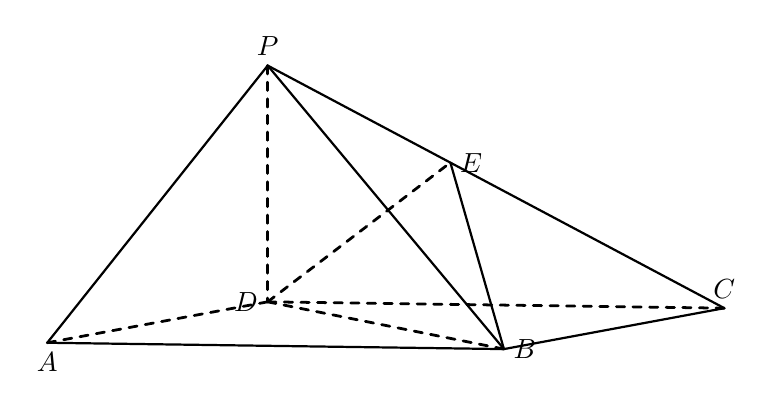
\begin{tikzpicture}[
    scale=1.5,
    line join=round,
    line cap=round,
    >=stealth,
    x={(-0.5cm,-0.2cm)},
    y={(1cm,0cm)},
    z={(0cm,1cm)},
    declare function={sqrt3=1.732;}
]
% 你的图形代码
\coordinate (D) at (0,0,0);
\coordinate (A) at ({sqrt3},-1,0);
\coordinate (B) at (2,3,0);
\coordinate (C) at (0.268,4,0);
\coordinate (P) at (0,0,2);

\draw[dashed,line width=1.0pt] (P) -- (D);
\draw[thick] (P) -- (A);
\draw[thick] (P) -- (B);
\draw[thick] (P) -- (C);
\draw[thick] (B) -- (C);
\draw[thick] (A) -- (B);

\draw[dashed,line width=1.0pt] (D) -- (A);
\draw[dashed,line width=1.0pt] (D) -- (B);
\draw[dashed,line width=1.0pt] (D) -- (C);

\node[left] at (D) {$D$};
\node[below] at (A) {$A$};
\node[right] at (B) {$B$};
\node[above] at (C) {$C$};
\node[above] at (P) {$P$};

\coordinate (E) at ($(P)!0.4!(C)$);
\draw[dashed,line width=1.0pt] (D) -- (E);
\draw[thick] (B) -- (E);
\node[right] at (E) {$E$};

\end{tikzpicture}

\end{problem}
\pagebreak

\begin{problem}
已知数列 $\{a_{n}\}$ 的前 $n$ 项和为 $S_{n}, a_{1} = 1$ 且 $a_{n+1} = S_{n} + 1 (n \in \mathbf{N}^{*})$。
\begin{enumerate}
\item 求数列 $\{a_{n}\}$ 的通项公式;
\item 在 $a_{n}$ 与 $a_{n+1}$ 之间插入 $n$ 个数,使这 $n+2$ 个数组成一个公差为 $d_{n}$ 的等差数列。
\begin{enumerate}
\item 记 $b_{n} = \frac{1}{d_{n}}$,求数列 $\{b_n\}$ 的通项公式 $b_{n}$
\item 求数列 $\{b_n\}$ 的前 $n$ 项和 $T_{n}$
\end{enumerate}
\end{enumerate}
\end{problem}
\vspace{600}


\begin{problem}
在平面直角坐标系 $xOy$ 中,对于任意一点 $P(x,y)$,总存在一个点 $Q(x', y')$ 满足关系式 $\varphi: \begin{cases} x' = \lambda x, \\ y' = \mu y, \end{cases} (\lambda > 0, \mu > 0)$,则称 $\varphi$ 为平面直角坐标系中的伸缩变换。
\begin{enumerate}
\item 在同一直角坐标系中,求平面直角坐标系中的伸缩变换 $\varphi_{1}$,使得圆 $x^{2} + y^{2} = 8$ 变换为椭圆 $\frac{x^2}{2} + y^2 = 1$;
\item 已知曲线 $E_{1}$ 经过平面直角坐标系中的伸缩变换 $\varphi_{2}:\left\{ \begin{array}{l}x^{\prime} = 2x,\\ y^{\prime} = y \end{array} \right.$ 得到的曲线是 $E_{2}: \frac{x^{2}}{16} -y^{2} = 1$,且 $E_{1}$ 与 $x$ 轴有 $A,B$ 两个交点($A$ 在 $B$ 的左侧),过点 $(4,0)$ 且斜率为 $k$ 的直线 $l$ 与 $E_{1}$ 在 $y$ 轴右侧有 $H,K$ 两个交点。
\begin{enumerate}
\item 求 $k$ 的取值范围;
\item 若直线 $AH, BH, BK$ 的斜率分别为 $k_{1}, k_{2}, k_{3}$,证明:$k_{2}(k_{1} + k_{3})$ 为定值。
\end{enumerate}
\end{enumerate}
\end{problem}
\vspace{600}


\end{document}
